\subsection{Gene density and seed fragments}

\begin{definition}{Contig gene density}{contig_gene_density}
  Let \(c \in \Contigs{}\) be a contig.
  By \(\gd{c} \in [0, 1]\) we denote its gene density:
  \[
    \gd{c} = \frac{ \ncovnuc{c} }{ |c| }
  \]
  Where \(\ncovnuc{c}\) is the number of nucleotides of contig \(c\) covered by gene mapping matches.
\end{definition}

\begin{definition}{Fragment gene density}{frag_gene_density}
  \begin{newfeatbox}
    We recompute the gene density of the fragments according to the position of the fragments on the contigs.
  \end{newfeatbox}

  Let \(i\) be a pangenome fragment.
  By \(\gd{i} \in [0, 1]\) we denote its gene density:
  \[
    \gd{i} = \frac{1}{ |i| \times |\Contigs{}(i)| } \sum_{\substack{
        c \in \Contigs{}(i) \\
    }} \ncovnuc{c}(\fcstart{i}{c}, \fcend{i}{c})
  \]
  Where \(\ncovnuc{c}(\fcstart{i}{c}, \fcend{i}{c})\) is the number of nucleotides of contig \(c\) covered by gene mapping matches between positions defined by \(i\) on \(c\).
\end{definition}

\subsubsection{Seed fragment candidates}

\begin{notebox}
  A first solution can be using the same computation as in PlasBin-flow, however, a gene can be contained in a contig, while a gene can correspond to a sequence of fragments.
  \Cref{fig:seed_frag-split_plasmid_gene} illustrates the situation.
\end{notebox}

We map genes from a plasmid gene reference database to the contigs.
As in~\cite{manePlasBinflowFlowbasedMILP2023}, we determine a pair of thresholds \((l, gd)\) maximizing the expression \(SP - NPS\) (see the description in the paper).
However, as the length and the gene density distributions differ between the assembled reference read dataset and the pangenome fragments, we normalize each threshold according to the distributions difference (according to the medians \(m\) and \(m'\)):

\[
  (l', gd') = \parenth*{\frac{m'}{m} l, \frac{m'}{m} gd}
\]

Thus, a fragment \(i \in \Fragments{}\) is in the seed fragment set \SeedFrags{} if, and only if \(|i| \geq l'\) and \(\gd{i} \geq gd'\).

\begin{newfeatbox}
  Here we take care of normalizing according the distribution of the parameters we filter (not done in PlasBin-flow)
\end{newfeatbox}

\begin{figure}[htb]
  \centering
  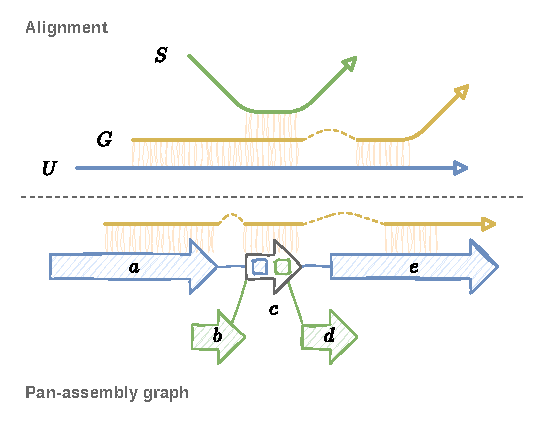
\includegraphics[width=0.6\linewidth]{pan-assembly_graph/img/seed_fragments-split_plasmid_gene.pdf}
  \figurecaption{The effect of fragmentation on plasmid gene mapping.}{%
    The top figure part represents a plasmid gene \(G\) (in orange) that partially maps onto Unicycler contig \(U\) (in blue) and SKESA contig \(S\) (in green).
    The bottom part illustrates the resulting pan-assembly subgraph, where fragments \(a\), \(c\) and \(e\) are defining contig \(U\), while fragments \(b\), \(c\), \(d\) are defining contig \(S\).
  }\label{fig:seed_frag-split_plasmid_gene}
\end{figure}